\documentclass{beamer}
\usetheme{CambridgeUS}

\usepackage[utf8]{inputenc}
\usepackage{tfrupee}
\usepackage{enumitem}
\usepackage{amsmath}
\usepackage{amssymb}
\usepackage{graphicx}
\usepackage{mathtools}
\providecommand{\sbrak}[1]{\ensuremath{{}\left[#1\right]}}
\providecommand{\lsbrak}[1]{\ensuremath{{}\left[#1\right.}}
\providecommand{\rsbrak}[1]{\ensuremath{{}\left.#1\right]}}
\providecommand{\brak}[1]{\ensuremath{\left(#1\right)}}
\providecommand{\lbrak}[1]{\ensuremath{\left(#1\right.}}
\providecommand{\rbrak}[1]{\ensuremath{\left.#1\right)}}
\providecommand{\cbrak}[1]{\ensuremath{\left\{#1\right\}}}
\providecommand{\lcbrak}[1]{\ensuremath{\left\{#1\right.}}
\providecommand{\rcbrak}[1]{\ensuremath{\left.#1\right\}}}
\newcommand{\myvec}[1]{\ensuremath{\begin{pmatrix}#1\end{pmatrix}}}
\let\vec\mathbf


\title{Assignment 8}
\author{Himanshu Kumar Gupta(AI21BTECH11012)}

\begin{document}
\begin{frame}
\maketitle
\end{frame}
\begin{frame}{Contents}
\tableofcontents  
\section{Question}
\end{frame}
\begin{frame}{Question}
    Let x be a negative binomial random variable with parameters r and p. Show that as $p \to 1$ 
and $r\to \infty$ such that $r\brak{1 - p}\to \lambda$, a constant, then
\begin{align}
    \Pr\brak{x=n+r}\to e^{-\lambda}\frac{\lambda^n}{n!}   
  \nonumber\\
  \text{where n=0,1,2,...}   \nonumber
\end{align}
\end{frame}
\section{Solution}
\begin{frame}{Solution}
We know that
\begin{align}
    \Pr\brak{X=k}=\binom{k-1}{r-1}p^rq^{k-r}
   \\ \text{where k=r,r+1,...}\nonumber
\end{align}



   \end{frame}
\begin{frame}
Let k=n+r so that
\begin{align}
 \Pr\brak{X=n+r}&=\binom{n+r-1}{r-1}p^r q^{n}    \nonumber\\
&\text{where n=0,1,2,...}\nonumber\\
  & =\frac{\brak{n+r-1}!}{\brak{n}!\brak{r-1}!}p^r\brak{1-p}^n  \nonumber\\
   & =\frac{(n+r-1)(n+r-2)...(r)}{n!}\frac{\cbrak{r(1-p)}^n p^r}{r^n}  \nonumber\\
   & =\frac{\lambda^n}{n!}\cbrak{\brak{1+\frac{n-1}{r}}...\brak{1}}\cbrak{1-\frac{r\brak{1-p}}{r}}^r   \nonumber\\
   & =\frac{\lambda^n}{n!}\cbrak{\prod_{k=1}^{n}\brak{1+\brak{n-k}{r}}}\brak{1-\frac{\lambda}{r}}^r
\end{align}
    
\end{frame}
\begin{frame}
    Now,
    \begin{align}
        \lim_{r\to \infty}\Pr\brak{X=n+r}&=\frac{\lambda^n}{n!}\cbrak{\lim_{r\to\infty}\prod_{k=1}^{n}\brak{1+\frac{n-k}{r}}}\lim_{r\to\infty}\brak{1-\frac{\lambda}{r}}^r     \nonumber  \\
        &=\frac{\lambda^n}{n!}\times1\times e^{-\lambda}
    \end{align}
    So,
    \begin{align}
         \Pr\brak{x=n+r}\to e^{-\lambda}\frac{\lambda^n}{n!} 
  \nonumber
    \end{align}
\centerline{ as $p \to 1$ 
and $r\to \infty$}
\end{frame}
\begin{frame}
    \begin{figure}[htb!]

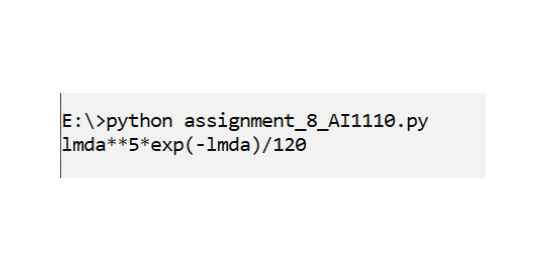
\includegraphics[width=13cm]{figures/assign_8_python.png}
\caption{python output}
\end{figure}
\end{frame}
\end{document}
